\documentclass[../main.tex]{subfiles}

Este capítulo aborda el diseño e implementación del software. En primer lugar se explicará el esquema seguido junto a las motivaciones de cada decisión de diseño tomada. Se presentarán los diferentes bloques en los que se organiza el código, que a su vez se desarrollarán en las secciones sucesivas. \\

\section{Diseño} \label{section:dis-dis}
La aplicación ha sido diseñada desde el primer momento teniendo en cuenta los objetivos iniciales y requisitos del proyecto. A lo largo de esta sección, se harán múltiples referencias a los objetivos introducidos durante la Sección \ref{section:intro-objetivos}. \\
En la aplicación se integran múltiples funciones como la configuración en función de la aeronave, la programación de misiones, el seguimiento y cumplimiento de las mismas y la visualización de los sensores a bordo, entre otras funciones. \\
Existen diferentes formas de agrupar o segmentar la aplicación para un mejor análisis del código y una mejor comprensión del diseño realizado. En primer lugar, se presenta un diseño que agrupa la aplicación en bloques o módulos con funciones bien distinguidas entre sí. Se distinguen los siguientes grandes bloques:

\begin{itemize}
    \item \textbf{Interfaz gráfica:} Está compuesto por una serie de ventanas, \emph{widgets} y herramientas que dan soporte al resto de bloques y que permiten al usuario interactuar con la aplicación. La Sección \ref{section:dis-gui} muestra el diseño e implementación seguida y explica más en detalle el bloque.
    \item \textbf{Mapas:} Se compone de una serie de clases que permiten la visualización e interacción con los mapas. Utiliza un sistema de mapeado basado en teselas que aligera la navegación a través del mapa. Dispone de diferentes fuentes cartográficas que permiten visualizar diferentes mapas sobre la misma herramienta. Durante la Sección \ref{section:dis-map} se detalla en profundidad aspectos relacionados con el diseño e implementación de este bloque. 
    \item \textbf{Misiones:} Este bloque engloba las clases que intervienen en la creación de misiones. Se distinguen dos tipos de misión: por polilínea y por patrón. Más detalles y cuestiones relacionadas con el diseño e implementación se aportan en la Sección \ref{section:dis-mision}.
    \item \textbf{MAVLink Driver:} Este último bloque contiene toda vía de comunicación con la aeronave. Es el encargado de traducir las acciones lanzadas a través de la aplicación a mensajes MAVLink que la aeronave comprende. Este bloque es una evolución del código desarrollado por J.A. Fernández durante su proyecto fin de carrera \cite{pfc-jose}. Se aportan más detalles en la Sección \ref{section:dis-driver} sobre el diseño e implementación del \emph{driver}.
\end{itemize}

En la Figura \ref{fig:esquema-bloques} se observa como configuran la aplicación los diferentes bloques presentados. En la parte superior de la figura se encuentra el \emph{front-end} de la aplicación, que está compuesto en su totalidad por la interfaz de usuario (GUI, \emph{Graphical User Interface}). En una segunda capa se encuentra la parte lógica de la aplicación que se divide en distintos bloques, principalmente compuestos por el sistema de mapeado y el creador de misiones. En una tercera y última capa se encuentran una serie de servicios que aportan comunicación a la aplicación con el exterior. Se destacan dos servicios principales, los mapas web y el \emph{driver} de MAVLink. Estas dos capas internas conforman el \emph{back-end} de la aplicación. \\

\begin{figure}[ht]
    \centering
    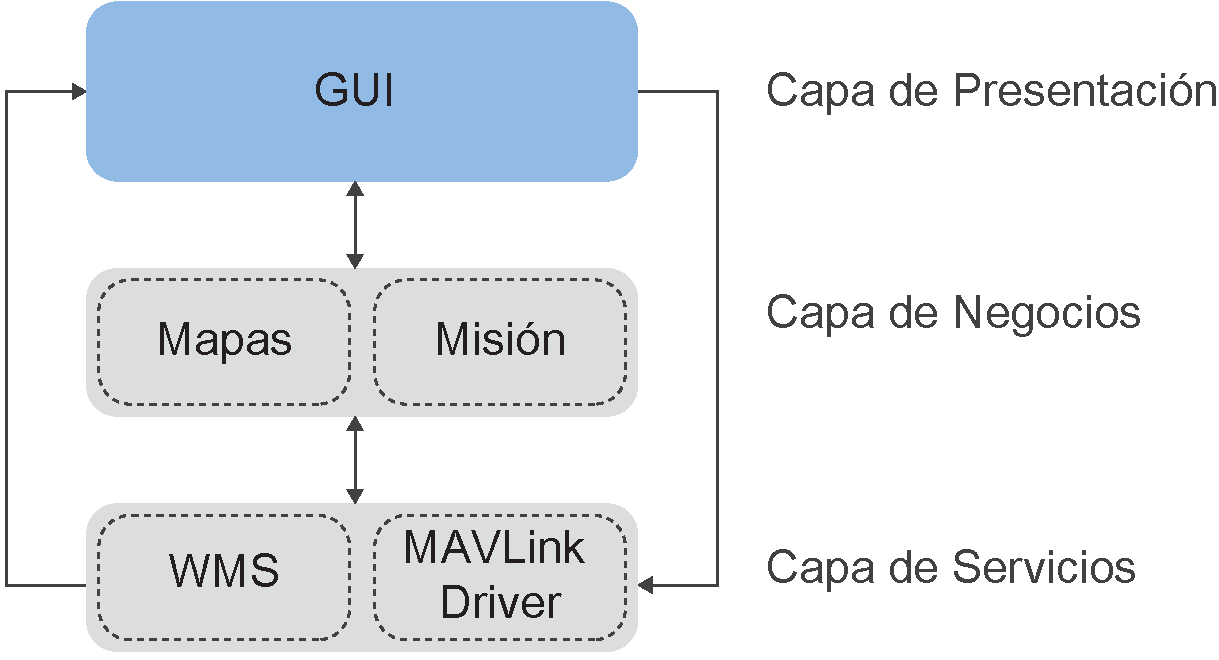
\includegraphics[width=0.8\textwidth]{esquema-bloques.pdf}
    \caption{Capas que componen la aplicación.}
    \label{fig:esquema-bloques}
\end{figure}

Esta estructura en capas que se presenta ha permitido dividir el problema inicial en subproblemas, para afrontarlos individualmente de una forma más sencilla. Además esta estructura al ser tan gráfica permite entender los diferentes módulos y su función dentro de la aplicación.

Por otro lado, desde un punto de vista de ejecución la aplicación contiene cuatro hilos. Cada uno de estos hilo realiza tareas diferentes en uno o en varios de los bloques ya explicados. Previo paso a la descripción de los hilos de ejecución, es necesario introducir las interfaces utilizadas en la aplicación. Son cuatro, \emph{Pose3D}, \emph{NavData}, \emph{mission} y \emph{extra}, todas reciclajes de las antiguas interfaces de JdeRobot con ICE \cite{pfc-jose}. \\

\begin{itemize}
    \item \textbf{Pose3D:} Contiene los datos de posición en el espacio de la aeronave y su orientación. La orientación en el espacio es expresada mediante el uso de cuaterniones.
    \item \textbf{NavData:} Sirve datos secundarios de actuación como velocidades lineales o angulares o el estado de la batería.
    \item \textbf{mission:} Almacena los puntos de la misión con una posición en el espacio para cada uno.
    \item \textbf{extra:} Permite distinguir los puntos y asociar acciones de despegue y aterrizaje a puntos concretos.
\end{itemize}

A continuación se presentan estos hilos de ejecución con una breve descripción de los mismos: 

\begin{itemize}
    \item \textbf{Hilo principal:} Tiene asociado las principales acciones de la aplicación. Las diferentes ventanas y herramientas surgen de él, al igual que el sistema de mapeado y el creador de misiones.
    \item \textbf{Handler de mensajes:} Se encarga de escuchar y leer los mensajes enviados por la aeronave. Tras leer los mensajes recibidos, extrae la información relevante de los mismos y escribe esta información sobre las dos interfaces.
    \item \textbf{Hilo de navegación:} Se encarga de recoger los datos de navegación leyendo del interfaz \emph{NavData} para actualizar los sensores de navegación y otros valores importantes sobre el estado de navegación de la aeronave.
    \item \textbf{Hilo de posición:} De forma similar al hilo anterior, lee el interfaz \emph{Pose3D} y actualiza la posición de la aeronave sobre el mapa de la aplicación.
\end{itemize}

Sobre los hilos de ejecución es importante mencionar que no todos se lanzan al ejecutar la aplicación. Al inicio de la ejecución se crean tres hilos, el principal, el de navegación y el de posición, y durante el establecimiento de conexión con la aeronave se genera el \emph{handler}. Sin embargo, tanto el hilo de navegación como el de posición se encuentran latentes o inactivos hasta el establecimiento de conexión. Se darán más detalles sobre su funcionamiento durante la sección \ref{section:dis-driver}.

% diseño de caja negra, inputs and outputs

Por último, y previo paso a la vista en detalle de cada bloque, se presenta una figura (Fig. \ref{fig:esquema-clases}) con la estructura general de clases que contiene la aplicación. Esta figura contiene toda la información hasta ahora mencionada sobre el diseño de la aplicación: bloques, hilos de ejecución e interfaces. Esta figura supone una vista en conjunto cuya intención es proveer al lector de una visión global detallada sobre el software previo a ese análisis pormenorizado sobre cada uno de los bloques.

\begin{figure}[h]
    \centering
    \includegraphics[width=\textwidth]{esquema-clase-capas.pdf}
    \caption{Esquema de clases del sistema.}
    \label{fig:esquema-clases}
\end{figure}

También cabe destacar que este software no ha sido desarrollado en su totalidad por el autor, sino que hace uso de cierta infraestructura anteriormente desarrollada. Además del \emph{driver} de comunicaciones MAVLink (desarrollado por J.A. Fernández \cite{pfc-jose}) y las interfaces de JdeRobot (\emph{NavData} y \emph{Pose3D}), también se hace uso de una librería de sensores que permite visualizar de forma más realista los datos de navegación \cite{qfi-python}.
A continuación, cada uno de los bloques de software de la aplicación se detalla en las sucesivas secciones de este capítulo.

\section{Interfaz Gráfico de Usuario} \label{section:dis-gui}
La interfaz gráfica de usuario (GUI, \emph{Graphical User Interface}) se compone de una serie de objetos gráficos que presentan la información y acciones disponibles al usuario. Se organiza en un conjunto de ventanas y \emph{widgets}. La aplicación dispone de una ventana principal, cuatro ventanas secundarias y varias ventanas de carga y guardado. También se hace uso de diálogos para mostrar mensajes al usuario. \\

\subsection{Ventana principal}
La ventana principal se divide en cinco diferentes pestañas según las funcionalidades de la aplicación. Estas pestañas coinciden con los objetivos secundarios presentados durante la Sección \ref{section:intro-objetivos} y reciben el nombre de \emph{Setup} para la caracterización de la aeronave y la carga de pago, \emph{Mission} para la creación de misiones de vuelo automático, \emph{Checklist} para la comprobación de pre-vuelo, \emph{Follow} para el seguimiento de vuelo y \emph{Log} para el análisis de datos post-vuelo. El la Figura \ref{fig:setup} se puede observar la primera pestaña de la aplicación, tal y como se encuentra recién iniciada la aplicación. \\

\begin{figure}[h]
    \centering
    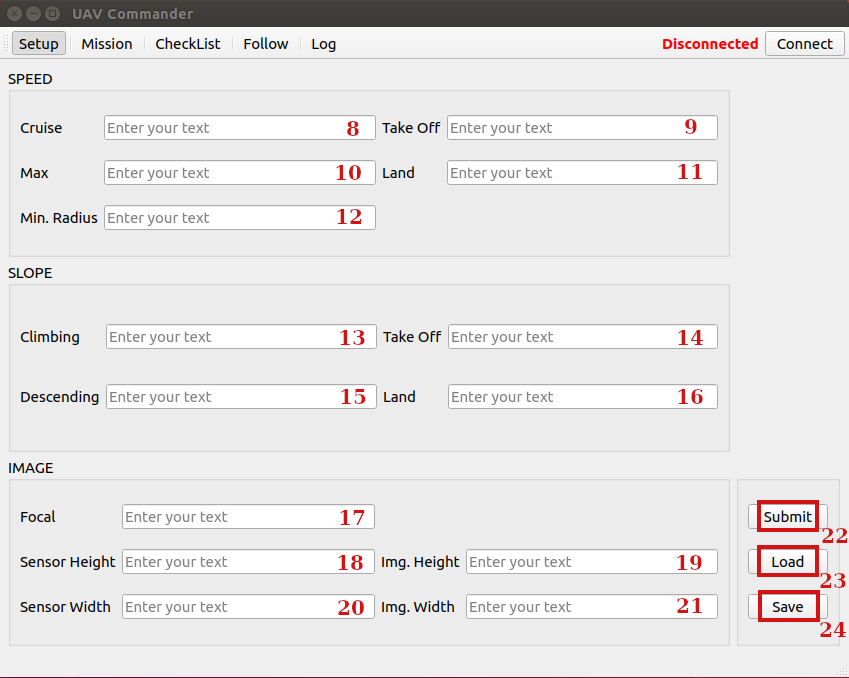
\includegraphics[width=0.8\textwidth]{screenshots/setup.png}
    \caption{Ventana principal con la pestaña \emph{Setup} activa.}
    \label{fig:setup}
\end{figure}

Esta estructura se ha conseguido haciendo uso de diferentes \emph{QWidgets} asociado a cada una de las pestañas organizados a través de un \emph{QStackedWidget} y una serie de \emph{QAction} que permiten activar y visualizar un \emph{QWidget} u otro. A continuación se muestra un fragmento del código (Cód. \ref{listing:vent-ppal}) donde se observa la estructura utilizada.

\begin{listing}[h]
\begin{minted}[frame=lines, framesep=2mm, baselinestretch=1.2, bgcolor=LightGray, fontsize=\footnotesize, linenos]{python}
def __init__(self, *args, **kwargs):
    
    ....
    self.widgets = QStackedWidget()
    self.widgets.addWidget(MySetupWidget(self))
    self.widgets.addWidget(MyMissionWidget(self))
    self.widgets.addWidget(MyChecklistWidget(self))
    self.widgets.addWidget(MyFollowWidget(self))
    self.widgets.addWidget(MyLogWidget(self))
    
    self.setCentralWidget(self.widgets)

    toolbar = QToolBar()
    self.addToolBar(toolbar)

    self.setup_action = QAction("Setup", self)
    self.setup_action.triggered.connect(self.onSetupToolBarClick)
    self.setup_action.setCheckable(True)
    toolbar.addAction(self.setup_action)

    toolbar.addSeparator()
    ....
    
def onSetupToolBarClick(self):
    self.setup_action.setChecked(True)
    self.mission_action.setChecked(False)
    self.checklist_action.setChecked(False)
    self.follow_action.setChecked(False)
    self.log_action.setChecked(False)

    self.widgets.setCurrentIndex(0) # Fija el widget visible 
    
    
\end{minted}

\caption{Estructura de pestañas en la ventana principal.}
\label{listing:vent-ppal}
\end{listing}

Para cada una de las pestañas se crea una clase nueva a través de una herencia simple de la clase abstracta \emph{QWidget}. De esta forma, las clases creadas comparten los atributos y procedimientos de la clase base, pudiendo ser personalizadas para que cumplan sus requisitos individuales. \\

\subsection{Ventanas secundarias}

Entre las ventanas secundarias anteriormente mencionadas se encuentran la ventana de configuración, la ventana de carga de mapa local, la ventana de sensores y la ventana de puntos de paso en la misión. En la Figura \ref{fig:vent-sec} se pueden observar alguna de estas ventanas secundarias.

\begin{figure}[h]
    \centering
    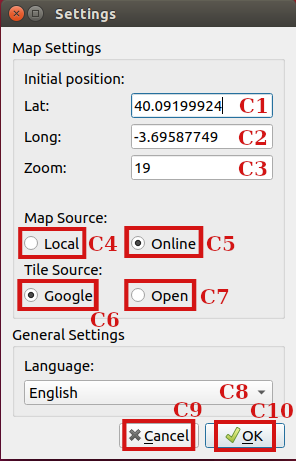
\includegraphics[width=0.4\textwidth]{screenshots/settings.png}
    \caption{Ventana secundaria de configuración.}
    \label{fig:vent-sec}
\end{figure}

En la ventana de configuración se pueden observar algunos de los datos persistentes entre  ejecuciones. El almacenamiento persistente y la recuperación de la configuración previa se consigue gracias a la clase \emph{QSettings} que proporciona Qt5. Además, en esta ventana se puede observar también la posibilidad de cambiar el idioma de la interfaz durante la ejecución. Esta traducción dinámica es posible gracias a la clase \emph{QTranslator} de Qt5 que permite cargar ficheros de traducción previamente generados y realizar las traducciones. Actualmente la aplicación se encuentra disponible en castellano e inglés.

\section{Sistema de Mapeado} \label{section:dis-map}
El bloque de mapas permite la visualización e interacción a través de la interfaz gráfica de la superficie terrestre. Son muchos los actores que entran en juego y que permite su funcionamiento. La principal herramienta sobre la que trabajan el resto de herramientas es una \emph{QGraphicsScene} (escena). Esta clase proporciona una superficie para desplegar y administrar una serie de elementos gráficos 2D. \\
Entre las diferentes acciones de las que se encarga el sistema se distinguen la visualización, la obtención de la imagen, la conversión de coordenadas y el manejo de las interacciones del usuario. 

\subsection{Visualización del mapa}
Para dar soporte a la visualización del mapa a través de la interfaz gráfica no es suficiente con la escena. La clase \emph{QGraphicsView} proporciona un \emph{widget} para mostrar el contenido de una \emph{QGraphicsScene}. Así pues, la \emph{QGraphicsView} (vista) sirve de nexo entre la escena y la interfaz gráfica. Son dos las vistas utilizadas sobre una única escena, pues en dos pestañas es necesario visualizar el mapa, en \emph{Mission} y en \emph{Follow}. \\
Por otro lado, con el objetivo de agilizar la visualización y la navegación a través del mapa se presenta un mapa en mosaico, compuesto por un número fijo de teselas o imágenes.
Así pues, se introduce la primera herramienta bajo la escena, las teselas. Las teselas constituyen un grupo de elementos gráficos 2D que son gobernados bajo las mismas reglas. Estos elementos gráficos son en su totalidad imágenes con una posición asociada que permite la construcción del mosaico. En esta primer versión del software las teselas utilizadas son nueve, aunque se está trabajando para que el número utilizado sea variable permitiendo así modificar el tamaño de la escena y dar más versatilidad al sistema de mapeado. \\

% figura de estructura de view y scene

% figura de estructura de teselas

\subsection{Obtención de la imagen}
El sistema de mapas soporta diferentes formatos u orígenes de las imágenes. Actualmente existen tres alternativas para visualizar el mapa:

\begin{itemize}
    \item \textbf{Imagen satélite de Google Earth:} Se obtiene a través del servidor de teselas de Google (GTS, \emph{Google Tile Server}).
    \item \textbf{Imagen de Open Maps:} Se obtiene a través del servidor de teselas de Open Street Maps.
    \item \textbf{Imagen satélite del IGN:} Se obtiene cargando archivos locales con fotografías geo-referenciadas, como los archivos ECW o TIFF. Estos archivos provienen del Instituto Geográfico Nacional a través del programa nacional de ortofotografía aérea (PNOA). 
\end{itemize}

Paralelamente al sistema de teselas existe otra herramienta que permite el uso de mapas locales. Esta herramienta permite leer y guardar información relevante sobre los archivos geo-referenciados (ECW o TIFF) para extraer así las teselas sobre la imagen completa, que serán utilizadas por la herramienta de teselas anterior. \\
En la Figura \ref{fig:teselas-alternat} se pueden comparar las tres opciones con las que se puede visualizar el mapa. Las imágenes mostradas corresponden a una tesela de tamaño 256x256 píxeles sobre la misma posición.

\begin{figure}[!ht]
    \begin{subfigure}{0.33\textwidth}
        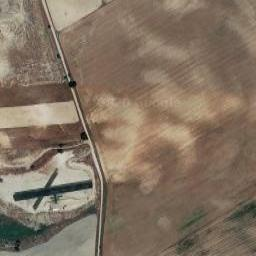
\includegraphics[height=4cm, width=0.9\linewidth]{tesela-google.jpeg}
        \caption{Tesela de Google Earth.}
        \label{fig:tesela-google}
    \end{subfigure}%
    \hfill
    \begin{subfigure}{0.33\textwidth}
        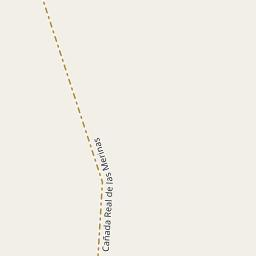
\includegraphics[height=4cm, width=0.9\linewidth]{tesela-open.jpeg}
        \caption{Tesela de Open Maps.}
        \label{fig:tesela-open}
    \end{subfigure}%
    \hfill
    \begin{subfigure}{0.33\textwidth}
        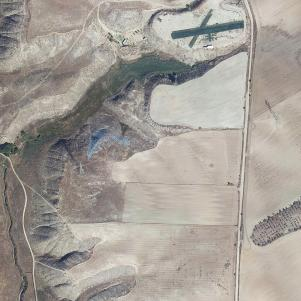
\includegraphics[height=4cm, width=0.9\linewidth]{tesela-local.jpeg}
        \caption{Tesela de mapa local.}
        \label{fig:tesela-local}
    \end{subfigure}%
     
    \caption{Diferentes teselas disponibles para visualizar el mapa.}
    \label{fig:teselas-alternat}
\end{figure}

La obtención de la imagen depende del tipo de mapa a visualizar. En la Figura \ref{fig:secuencia-mapas} se representa la secuencia de llamadas necesaria para obtener obtener una escena. \\

De la secuencia de llamadas se puede deducir diferentes aspectos relevantes de la obtención de mapas. En primer lugar, la aplicación utiliza una caché para reducir la latencia y agilizar así la obtención del mosaico. Esto es debido a que los servicios WMS o la lectura de grandes ficheros geo-referenciados son procesos lentos y pesados. \\
También se puede observar que los primeros pasos para la obtención de las teselas son comunes, y solo en el último paso difieren los caminos según el \emph{source} (origen) introducido como parámetro. Además, la función \emph{get-scene()} llamará a \emph{get-pixmap()} tantas veces como teselas posea la escena. \\
Por último, para obtener una escena concreta es necesario conocer las coordenadas (\emph{x, y, z}), el origen (\emph{source}) y el desplazamiento del centro (\emph{cx, cy}). Las diferentes coordenadas utilizadas se explicarán en la siguiente subsección.

\begin{figure}[h]
    \centering
    \includegraphics[width=\textwidth]{obtencion-imagen.pdf}
    \caption{Secuencia de llamadas para obtener una escena concreta.}
    \label{fig:secuencia-mapas}
\end{figure}

\subsection{Conversión de coordenadas}
La conversión de coordenadas de latitud y longitud a píxeles en la escena es un proceso complejo e inexacto. El simple posicionamiento sobre el globo terrestre es una aproximación más o menos exacto según el datum utilizado. El geoide o el elipsoide seleccionado trata de aproximarse a la forma real del globo terráqueo o a una zona de la superficie de la Tierra. Desde 1984 el geoide utilizado de forma mundial es el WGS84. \\ 
En segundo lugar, la conversión de una esfera (o algo que se asemeja a una esfera) a un plano conlleva también otro error asociado. La proyección más utilizada mundialmente es la proyección de Mercator. \\
El siguiente paso supone la digitalización de la proyección. En función del tamaño y resolución del mismo, se asocia un nivel de zoom. Para un zoom igual a cero, la imagen tiene normalmente 256x256 píxeles, el siguiente nivel tiene 512x512 píxeles, y así sucesivamente. A este esquema de zooms se le conoce como los diferentes niveles de una pirámide. \\
Por último, cada nivel de la pirámide se divide en teselas de tamaño normalmente igual a 256x256 píxeles. De esta forma, para un zoom igual a uno habría cuatro diferentes teselas. Así pues, en la cima de la pirámide habría una tesela, en el siguiente nivel 4 teselas, 16 en el siguiente, etc. A cada una de estas teselas se le asocia un coordenada x y otra y para posicionarla sobre el mosaico. \\
En la Figura \ref{fig:esquema-teselas} se representa este sistema de conversión de coordenadas explicado. Este método es ampliamente utilizado y supone un estándar en cartografía para la representación de la superficie terrestre en prácticamente cualquier herramienta de navegación existente hoy en día. Al ser una solución muy utilizada, existen multitud de útiles que facilitan su uso. En la aplicación se ha creado un archivo \emph{TileUtils.py} que recoge estas funciones para la obtención y conversión de coordenadas.

\begin{figure}[h]
    \centering
    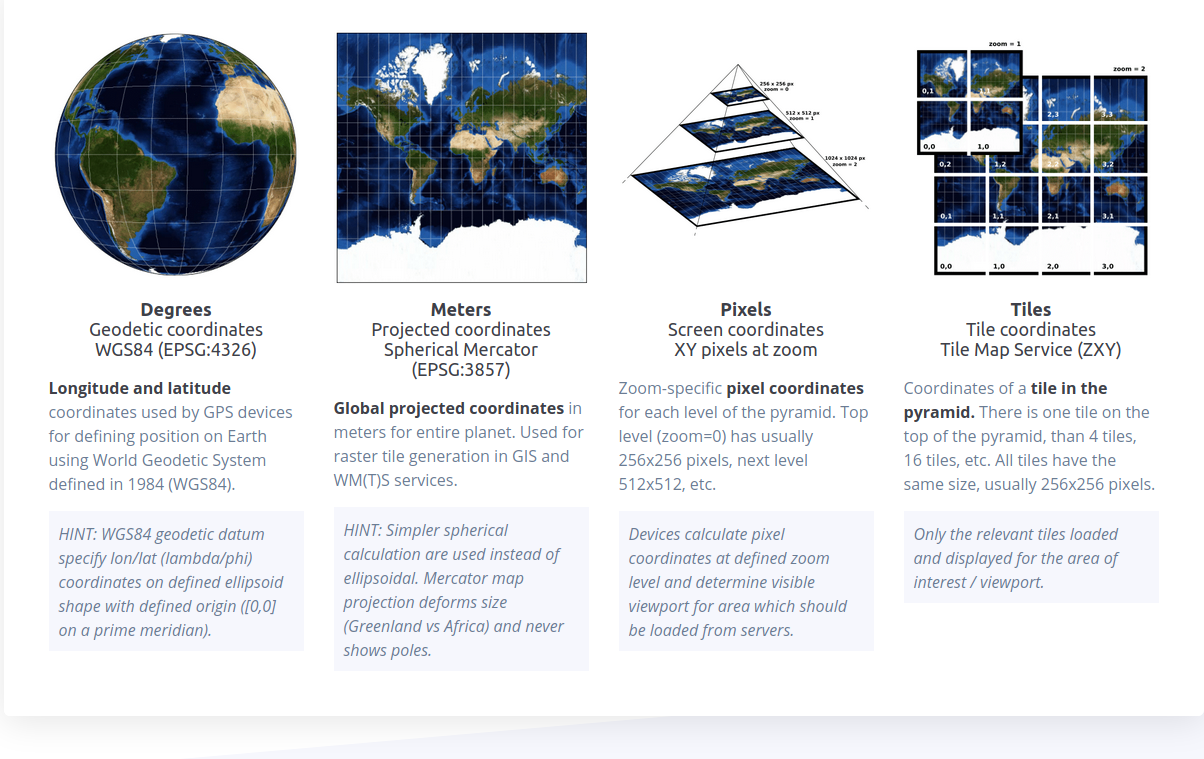
\includegraphics[width=\textwidth]{sist-coord.pdf}
    \caption{Esquema de conversión de coordenadas.}
    \label{fig:esquema-teselas}
\end{figure}

Debido al uso de una escena con un sistema de coordenadas propio es necesario una conversión más, entre el sistema de coordenadas de píxeles global y el sistema de píxeles local asociado a la escena. Estas funciones también se encuentran en el fichero de útiles \emph{TileUtils.py}.

\subsection{Interacción con el usuario}
El sistema de mapas soporta acciones típicas de navegación como el arrastre, el aumento o la disminución del mapa. Para esto, es necesario manejar las interacciones del usuario sobre el mapa. Se presenta entonces la tercera herramienta de la escena, un filtro que distingue entre los diferentes eventos recibidos por la escena y los redirige para tratarlos de forma diferente. A continuación se presenta un fragmento del código (Cód. \ref{listing:filter}) que se encarga de filtrar los diferentes eventos. \\


Los eventos filtrados son tres. En la línea 2 (Cód. \ref{listing:filter}) se detectan las pulsaciones de ratón, registrando la posición del mismo, mientras que en la línea 6 se detecta la posición en la que se suelta el pinchazo de ratón sobre la escena. Estas dos posiciones se comparan (línea 9), si son iguales, la acción realizada por el usuario se considera un clic y entonces el evento se trata como la suma de un nuevo punto de paso (línea 11). En cambio, si las posiciones detectadas entre pulsación y suelte son diferentes, la acción se considera un arrastre sobre el mapa mostrado, por lo que la escena se actualizará (línea 17). \\
Por otro lado, el la línea 20 se detectan los eventos relacionados con la rueda del ratón que se tratan como aumentos o disminuciones sobre el mapa. Además, cualquier otro evento sobre la escena sería fácilmente detectable y manejable modificando solamente el filtro. \\

\begin{listing}[h]
\begin{minted} [frame=lines, framesep=2mm, baselinestretch=1.2, bgcolor=LightGray, fontsize=\footnotesize, linenos]{python}

    def sceneEventFilter(self, source, event):
        if event.type() == QtCore.QEvent.GraphicsSceneMousePress:
            if event.button() == QtCore.Qt.LeftButton:
                self.initPos = event.scenePos()
                return True
        elif event.type() == QtCore.QEvent.GraphicsSceneMouseRelease:
            if event.button() == QtCore.Qt.LeftButton:
                self.pos = event.scenePos()
                if self.initPos == self.pos:
                    # Add waypoint
                    self.scene().addWayp(event.scenePos())
                else:
                    # Drag & Drop
                    
                    ....
                    
                    self.scene().updateScene(desp_tx, desp_ty, 
                                                desp_tz, cx, cy)
                self.initPos = None
                return True
        elif event.type() == QtCore.QEvent.GraphicsSceneWheel:
            # Zomm-in Zomm-out by mouse wheel movement
            
            ....

            self.scene().updateZoom(desp_tz, pos)
            return True

        # Another event
        return QGraphicsItem.sceneEventFilter(self, source, event) 

\end{minted}
\caption{Filtro de eventos de la escena.}
\label{listing:filter}
\end{listing}

Quedan por presentar dos herramientas más de la escena, una relacionada con la creación de misiones y otra con la representación del drone sobre la escena. Ambas serán explicadas en las siguientes secciones.

\section{Creador de Misiones} \label{section:dis-mision}
El creador de misiones permite, como su propio nombre indica, la creación y el envío de misiones a la aeronave a través del driver de MAVLink. Está íntimamente ligado a la escena, pues las misiones tienen un componente gráfico relevante que se representa sobre la escena.\\
Una misión se compone por los datos de configuración de la aeronave y la carga de pago y por una sucesión de puntos de paso. Ambos datos se pueden introducir a través de las dos primeras pestañas de la aplicación, \emph{Setup} y \emph{Mission}. Como es lógico pensar, los datos de configuración no dependen de la escena, mientras que la misión en sí misma (los puntos de paso) depende de la escena al tener elementos gráficos que representar. \\
Es importante destacar que ambas informaciones se pueden guardar en diferentes archivos de forma persistente en el disco. De la misma forma, estos archivos se pueden cargar en memoria. El formato seguido para la creación de estos ficheros de configuración y de misión es un formato plano de texto \cite{formato}. \\

\subsection{Tipos de misión}
Existen dos tipos de misiones, las misiones polilínea y las misiones de patrón. Las misiones polilínea se componen por una sucesión de puntos de paso y se crean introduciendo los diferentes puntos por orden. Es el tipo de misión más sencillo. Existen tres tipos de puntos, despegue, de paso o aterrizaje. Para introducir estos puntos existen dos posibilidades, bien pinchando sobre la escena directamente o introduciendo a mano una latitud y longitud deseada. En ambos casos es necesario introducir a mano la altura de vuelo deseada. En la Figura \ref{fig:mision-pol} se puede observar un ejemplo de una misión polilínea ya creada. \\
En cambio, las misión por patrón son más complejas. Se generan introduciendo los vértices de un polígono cerrado. Al igual que con la misión polilínea estos vértices pueden ser introducidos pinchando sobre el mapa o introduciendo la latitud y longitud del punto. El polígono puede ser irregular y convexo, la única restricción es que sea un polígono cerrado. Una vez creado el polígono se genera un algoritmo de barrido que recorre todo la superficie abarcada mediante una sucesión de puntos de paso. La altura introducida debe ser igual para todos los puntos de paso y se selecciona al introducir los vértices. En la Figura \ref{fig:mision-pat} se puede observar un ejemplo de una misión de patrón ya creada. Además, en el Código \ref{listing:alg-barrido} se muestra un fragmento del algoritmo de barrido creado para recorrer un superficie delimitada por una lista de vértices.

\begin{figure}[h]
    \begin{subfigure}{0.5\textwidth}
        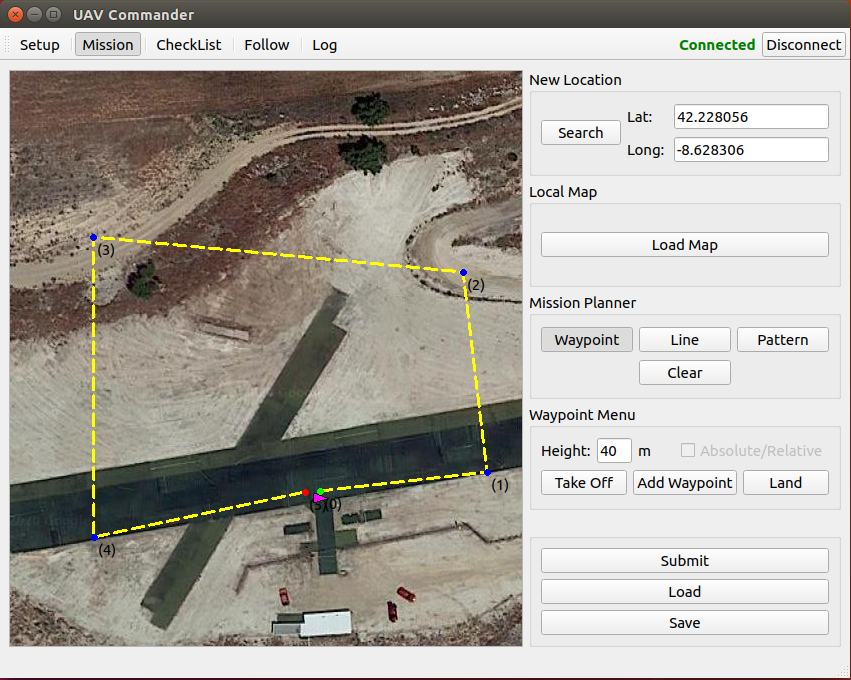
\includegraphics[height=6cm, width=0.9\linewidth]{screenshots/mission-wayp.png}
        \caption{Misión polilínea.}
        \label{fig:mision-pol}
    \end{subfigure}
    \begin{subfigure}{0.5\textwidth}
        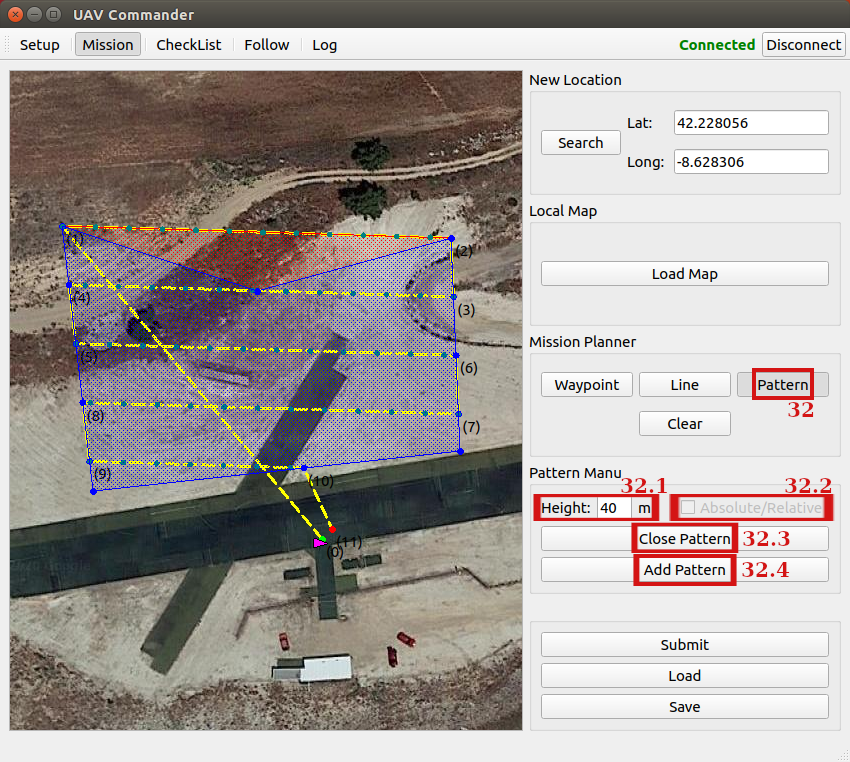
\includegraphics[height=6cm, width=0.9\linewidth]{screenshots/mission-pattern.png}
        \caption{Misión de patrón.}
        \label{fig:mision-pat}
    \end{subfigure}
     
    \caption{Tipos de misión disponibles.}
    \label{fig:tipos-mision}
\end{figure}

Los puntos de aterrizaje y despegue son algo diferentes a los punto de paso convencionales. Con respecto al despegue, la altura asociado a ese punto se corresponde con una altura de seguridad, la cual se debe haber sobrepasado para poder iniciar la misión y avanzar hacia el primer punto de paso. La senda de despegue se configura en línea recta según la orientación en el despegue. Para multicópteros esta senda es completamente vertical, mientras que para las aeronaves de ala fija se utilizará el valor asociado a la inclinación de despegue. \\
Por otro lado, el aterrizaje funciona también similar. La senda de aterrizaje se creará a través de dos puntos. El primero de ellos será el último punto de paso introducido y fijará la altura a la que se inicia la aproximación. El segundo punto fija el punto de aterrizaje y la orientación de la aproximación. Para multicópteros esta aproximación será vertical, mientras que para alas fija se utilizará el valor de la inclinación de aterrizaje introducida durante la caracterización de la aeronave. \\

La altura seleccionada para los puntos de paso o el barrido puede ser global o relativa. El término \emph{global} apunta a una altura de referencia constante (global) según el punto de despegue para toda la misión. En cambio, el término \emph{relativo} utiliza una referencia variable en función de la altitud del terreno en cada punto. \\
En las Figuras \ref{fig:tipos-mision} se pueden observar dos ventanas secundarias que muestran la lista de puntos de paso o vértices introducidos. Es a través de estas ventanas como se pueden añadir tanto los puntos de paso como los vértices a partir de su latitud y longitud. En una futura versión se planea introducir la posibilidad de modificar los puntos desde estas ventanas, aportando más versatilidad a esta herramienta. \\

\begin{longlisting}
\begin{minted} [frame=lines, framesep=2mm, baselinestretch=1.2, bgcolor=LightGray, fontsize=\footnotesize, linenos]{python}

    def calc_path(self):
        # Fija los parámetros iniciales del escaneo
        self.set_scan(self.p_init)

        # Primera pasada
        self.wayp.append(self.v_scan)
        self.calc_intermediates(self.v_scan, 
                    self.get_first_vertex(self.v_scan, self.l_scan))
        self.wayp.append(self.get_first_vertex(self.v_scan, self.l_scan))

        i = 1
        while True:
            # Calcula la siguiente pasada
            aux = self.get_next_aux(i) 
            # Comprueba si la pasada es válida
            vertexes_valid = self.get_valid_vertex(aux) 
            # Ordena los puntos de la pasada
            vertexes_valid = self.get_next_vertex(i, vertexes_valid, self.u_scan)

            if len(vertexes_valid) == 0: # FIN
                break
            elif len(vertexes_valid) == 1:
                self.wayp.append(vertexes_valid[0])
            elif len(vertexes_valid) >= 2:
                self.wayp.append(vertexes_valid[0]) # Siguiente pasada
                self.calc_intermediates(vertexes_valid[0], vertexes_valid[-1])
                self.wayp.append(vertexes_valid[-1])

            i = i + 1

\end{minted}
\caption{Algoritmo de barrido para las misiones de patrón.}
\label{listing:alg-barrido}
\end{longlisting}

\vspace{5mm}

Cierta parte de este bloque se integra como una herramienta dentro de la escena, pues toda la representación gráfica mediante puntos, líneas o polígonos cobra cierta relevancia a la hora de visualizar la misión que se está creando. Así pues, la cuarta herramienta de la escena se ha ido explicando a lo largo de esta sección.

\subsection{Captura de imágenes}
El uso principal del software es cartográfico, para ello, es necesario la toma de fotografías por parte de la aplicación. Esta funcionalidad solo estaría disponible para la misiones por patrón, que están ideadas para el escaneo de superficies. Este cálculo de posiciones de captura de imagen se realiza de forma automática a partir de los datos del sensor y la altura de vuelo. Estas posiciones son las calculadas por el procedimiento \emph{calc\_intermediates(init, end)} en la líneas 6 y 26 del Código \ref{listing:alg-barrido}. \\
El procedimiento anterior utiliza constantes de la misión para calcular la posición de captura. Estas constantes de misión son la distancia entre fotografías consecutivas ($fotobase$, Ec. \ref{eq:fotobase}) y entre pasadas de la aeronave ($espaciamiento$, Ec. \ref{eq:espaciamiento}), y dependen de los datos del sensor y la altura de vuelo \cite{otero2010fotogrametria}. Las ecuaciones que comandan estos valores son:

\begin{equation}
    fotobase = sh*(1-p\%)*E_v
    \label{eq:fotobase}
\end{equation}
    
\begin{equation}
    espaciamiento = sw*(1-q\%)*E_v
    \label{eq:espaciamiento}
\end{equation}

Siendo $sh$ y $sw$ el alto y ancho del sensor, $p$ y $q$ el solapamiento longitudinal y transversal de las fotografías, cuyos valores típicos en tanto por ciento suelen ser $p=60\%$ y $q=30\%$, y finalmente, $E_v$ la escala de vuelo, que se calcula siguiendo $E_v=H/f$, donde $H$ es la altura de vuelo y $f$ la distancia focal del sensor. \\
La comunicación MAVLink para la toma de fotografías se explicará en la siguiente sección junto con las principales comunicaciones de la aplicación.

\section{MAVLink Driver} \label{section:dis-driver}
El último bloque integra diferentes funciones que dependen directamente de la comunicación con la aeronave. El driver de comunicaciones es bidireccional, y sirve tanto para recibir como para enviar información a la aeronave. Una vez más, se quiere resaltar que este bloque parte del trabajo inicial de J.A. Fernández en su proyecto fin de carrera \cite{pfc-jose}. \\
Las diferentes funciones se pueden clasificar de la siguiente forma:

\begin{itemize}
    \item Establecimiento de conexión.
    \item Envío de misión.
    \item Control de vuelo: Navegación y sensores.
    \item Control de vuelo: Posicionamiento de aeronave.
    \item Otros: modo de vuelo, velocidad crucero, etc.
\end{itemize}

Las diferentes funcionalidades se analizarán una por una en las siguientes subsecciones.

\subsection{Establecimiento de conexión}
La conexión con la aeronave se establece gracias a la librería pyMavlink, que como se ha explicado durante el Capítulo \ref{chapter:infra}, propone una implementación del protocolo de comunicaciones MAVLink facilitando acciones como esta. \\
En el fragmento de código (Cód. \ref{listing:conexion}) se pueden observar los dos procedimientos principales. Cabe destacar que el establecimiento no solo implica atarse a una dupla IP-puerto, sino que también incluye la creación de un \emph{handler} que se encarga de recibir los mensajes de la aeronave.

\vspace{2mm}

\begin{longlisting}
\begin{minted}[frame=lines, framesep=2mm, baselinestretch=1.2, bgcolor=LightGray, fontsize=\footnotesize, linenos]{python}

def establishConnection(self):
    # Launch the MAVLink messages handler
    if self.connection == 0:
        print("New connection")
        self.connection = MAVLinkDriver.uav_connect("udp:127.0.0.1:14540") # SITL
        # self.connection = MAVLinkDriver.uav_connect("udpin:0.0.0.0:14550") # 3DRSolo

        msgHandler = threading.Thread(target=MAVLinkDriver.mavMsgHandler, args=(
                        self.connection, self.pose, self.navdata,
                        self.msg_handler_thread_kill_signal), name='msg_Handler')
        msgHandler.start()
    ....

def uav_connect(port, baudrate=None):
    master = mavutil.mavlink_connection(port, baudrate, autoreconnect=True)
    print('Connection established to device')
    heartbeat = master.wait_heartbeat()
    
    print("Heartbeat Received", heartbeat)

    # Set the complete set of commands
    master.mav.request_data_stream_send(master.target_system, 
                                             master.target_component,
                                             mavutil.mavlink.MAV_DATA_STREAM_ALL,
                                             RATE, 1)
    return master
    
\end{minted}
\caption{Establecimiento de conexión.}
\label{listing:conexion}
\end{longlisting}

\vspace{5mm}

El protocolo de conexión de MAVLink es muy sencillo y se basa en el envío de mensajes \emph{HEARTBEAT}. Se utiliza para anunciar la existencia de un sistema en la red MAVLink, junto con su identificación del sistema y componente, tipo de vehículo, tipo de autopiloto, estado y modo de vuelo. Los distintos componentes deben transmitir regularmente sus \emph{HEARTBEAT} y controlar los recibidos desde otros componentes y/o sistemas. La estructura del mensaje \emph{HEARTBEAT} se presenta en la Tabla \ref{table:heartbeat}. Para más detalles sobre el tipo y los valores asociados a cada campo, se recomienda visitar la documentación de MAVLink \cite{heartbeat}.

\begin{table}[H]
    \centering
    \begin{threeparttable}
        \begin{tabular}{l l l l}
            \toprule
            \thead{Campo} & \thead{Tipo} & \thead{Valores} & \thead{Descripción} \\
            
            \midrule
            type             & uint8\_t  & MAV\_TYPE       & Tipo de vehículo o componente. \\
            autopilot        & uint8\_t  & MAV\_AUTOPILOT  & Tipo de autopiloto. \\
            base\_mode       & uint8\_t  & MAV\_MODE\_FLAG & Mapa de bits del modo del sistema. \\
            custom\_mode     & uint32\_t &                 & Flags del autopiloto. \\ 
            system\_status   & uint8\_t  & MAV\_STATE      & Flags de estado del sistema. \\
            mavlink\_version & uint8\_t  &                 & Versión de MAVLink. \\
            \bottomrule
            \addlinespace[1ex]
        \end{tabular}
        
    \end{threeparttable}
    
    \caption{Mensaje \emph{HEARTBEAT} \cite{heartbeat}.}
    \label{table:heartbeat}
    \end{table}

Entre las tareas que realiza el \emph{handler} se encuentran el manejo de mensajes enviados por el autopiloto, el envío de los \emph{heartbeats} o el refresco de las interfaces \emph{Pose3D} y \emph{NavData} con datos de la aeronave. El Código \ref{listing:handler} recoge la implementación en código de estas tareas. Más adelante se explicarán también las funciones de las interfaces y el control de vuelo.

\begin{listing}[h]
\begin{minted} [frame=lines, framesep=2mm, baselinestretch=1.2, bgcolor=LightGray, fontsize=\footnotesize, linenos]{python}

def mavMsgHandler(master, pose, navdata, stop_event):
    lastSentHeartbeat = 0
    while not stop_event.isSet():
        msg = master.recv_msg()
        
        # send heartbeats to autopilot
        if time.time() - lastSentHeartbeat > 0.5:
            master.mav.heartbeat_send(mavlink2.MAV_TYPE_GCS, 
                            mavlink2.MAV_AUTOPILOT_INVALID, 0, 0, 0)
            lastSentHeartbeat = time.time()

            # refresh the attitude
            refreshAPMPose3D(master, pose)
            refreshAPMnavdata(master, navdata)

        elif msg is None or msg.get_type() == "BAD_DATA":
            time.sleep(0.01)
            continue

\end{minted}
\caption{Handler de conexión.}
\label{listing:handler}
\end{listing}

\subsection{Envío de misión}
El envío de misiones se realiza a través del protocolo de misiones que propone MAVLink. La Figura \ref{fig:protocol-mission} recoge un diagrama del protocolo, el cual ha sido sacado de la propia web de MAVLink \cite{protocol-mission}. \\

\begin{figure}[h]
    \centering
    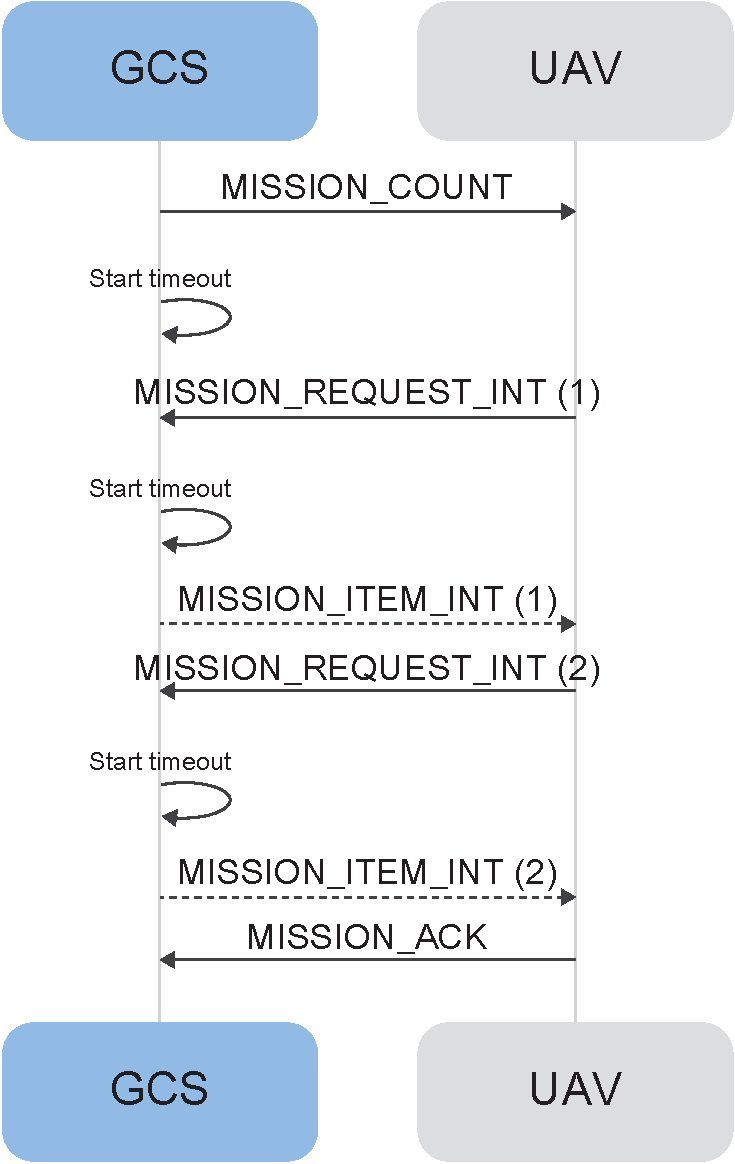
\includegraphics[width=0.5\textwidth]{prot-mision.pdf}
    \caption{Diagrama del protocolo de misiones de MAVLink.}
    \label{fig:protocol-mission}
\end{figure}

Los elementos que componen la misión se envían mediante mensajes \emph{MISSION\_ITEM}. La estructura de estos mensajes se representa en la Tabla \ref{table:mission-item}. Para más detalles sobre los campos del mensaje \cite{mission-item} o sobre otros mensajes que intervienen en el protocolo se recomienda visitar la documentación de MAVLink \cite{mavlink-msg}. \\
Estos mensajes encapsulan otros mensajes de tipo \emph{MAV\_CMD} o comandos. Algún ejemplo pueden ser los mostrados durante el Código \ref{fig:protocol-mission} en la línea 20 (\emph{MAV\_CMD\_NAV\_TAKEOFF}), línea 32 (\emph{MAV\_CMD\_NAV\_LAND}) o en la línea 43 (\emph{MAV\_CMD\_NAV\_WAYPOINT}), aunque existen muchos más \cite{mav-cmd-msg}. En función del comando especificado en el campo \emph{command} los siete parámetros tomarán un significado u otro. La Tabla \ref{table:comp-param} recoge las diferencias entre los tres comandos mencionados.

\begin{table}[H]
    \centering
    \begin{threeparttable}
        \begin{tabular}{l l l l}
            \toprule
            \thead{Campo} & \thead{Tipo} & \thead{Valores} & \thead{Descripción} \\
            
            \midrule
            target\_system    & uint8\_t  &                    & ID Sistema. \\
            target\_component & uint8\_t  &                    & ID Componente. \\
            seq              & uint16\_t &                    & Secuencia. \\
            frame            & uint8\_t  & MAV\_FRAME         & Sistema de coordenadas. \\ 
            command          & uint16\_t & MAV\_CMD           & Acción programada. \\
            current          & uint8\_t  &                    & Falso (0) o verdadero (1). \\
            autocontinue     & uint8\_t  &                    & Continuar automátic. \\
            param1           & float     &                    & PARAM1. \\
            param2           & float     &                    & PARAM2. \\
            param3           & float     &                    & PARAM3. \\
            param4           & float     &                    & PARAM4. \\
            x                & float     &                    & PARAM5 (Coord. X). \\
            y                & float     &                    & PARAM6 (Coord. Y). \\
            z                & float     &                    & PARAM7 (Coord. Z). \\
            mission\_type     & uint8\_t  & MAV\_MISSION\_TYPE & Tipo de misión. \\
            \bottomrule
            \addlinespace[1ex]
        \end{tabular}
        
    \end{threeparttable}
    
\caption{Mensaje \emph{MISSION\_ITEM} \cite{mission-item}.}
\label{table:mission-item}
\end{table}
    
\begin{table}[H]
    \centering
    \begin{threeparttable}
        \begin{tabular}{l l l l}
            \toprule
            \thead{Parámetros} & \thead{\emph{NAV\_TAKEOFF}} & \thead{\emph{NAV\_LAND}} & \thead{\emph{NAV\_WAYPOINT}} \\
            
            \midrule
            param1 & Cabeceo.  & Altura de decisión. & Tiempo de espera. \\
            param2 & -         & Modo de aterrizaje. & Radio aceptado. \\
            param3 & -         & -                   & radio de paso. \\
            param4 & Guiñada.  & Guiñada.            & Guiñada. \\
            param5 & Latitud.  & Latitud.            & Latitud. \\
            param6 & Longitud. & Longitud.           & Longitud. \\
            param7 & Altitud.  & Altitud.            & Altitud. \\
            \bottomrule
            \addlinespace[1ex]
        \end{tabular}
        
    \end{threeparttable}
    
\caption{Comparación entre parámetros de tres comandos \emph{MAV\_CMD\_}.}
\label{table:comp-param}
\end{table}

Entre los comandos que se pueden encapsular en los mensajes de misión destaca el usado para la toma de fotografías, \emph{MAV\_CMD\_DO\_SET\_CAM\_TRIGG\_DIST}. En la Tabla \ref{table:cmd-foto} se muestran los parámetros asociados a este comando. Este comando permite establecer una distancia de disparo donde la cámara captura cada vez que se supera esta distancia. El funcionamiento pues, es sencillo. Al inicio de la pasado se manda el mensaje de misión con la \emph{distancia} entre fotografías deseada, mientras que al final de la pasada se manda una \emph{distancia} nula para detener la captura de fotos. \\

\begin{table}[H]
    \centering
    \begin{threeparttable}
        \begin{tabular}{l l}
            \toprule
            \thead{Parámetros} & \thead{Descripción} \\
            
            \midrule
            Distancia   & Distancia de disparo. \\
            Obturación  & Tiempo de obturación. \\
            Disparo     & Disparo inmediato. \\
            param4      & - \\
            param5      & - \\
            param6      & - \\
            param7      & - \\
            \bottomrule
            \addlinespace[1ex]
        \end{tabular}
        
    \end{threeparttable}
    
\caption{Parámetros del comando \emph{MAV\_CMD\_DO\_SET\_CAM\_TRIGG\_DIST}.}
\label{table:cmd-foto}
\end{table}

Para la implementación del protocolo se parte de un pseudo-código propuesto por la Universidad de Colorado Boulder \cite{implem-prot}. Este boceto de implementación se adapta a la estructura de misiones de la aplicación, para construir los diferentes mensajes y el envío de misión. En el Código \ref{listing:protocol-mission} se recoge el resultado final de la implementación del protocolo.

\vspace{2mm}

\begin{longlisting}
\begin{minted} [frame=lines, framesep=2mm, baselinestretch=1.2, bgcolor=LightGray, fontsize=\footnotesize, linenos]{python}

def set_px4_mission(master, mission, extra, frame_type):
    wp = mavwp.MAVWPLoader()
    if frame_type:
        frame = mavutil.mavlink.MAV_FRAME_GLOBAL # 0
    else:
        frame = mavutil.mavlink.MAV_FRAME_GLOBAL_RELATIVE_ALT # 3

    seq = 1
    radius = 10
    pose3Dwaypoints = mission.getMission()
    N = len(pose3Dwaypoints)

    for i in range(N):
        if (i==0 and extra.takeOffDecision()):
            navData, is_img = pose3Dwaypoints[0]
            toff = mavutil.mavlink.MAVLink_mission_item_message(master.target_system,
                                                master.target_component,
                                                seq, frame,
                                                mavutil.mavlink.MAV_CMD_NAV_TAKEOFF,
                                                0, 1, 0, 0, 0, 0,
                                                navData.x, navData.y, navData.h)
            wp.add(toff)
            print("[MAVLink Driver] Takeoff to " + str(toff))
            seq += 1
            extra.setTakeoff(False)
        elif (i==N-1 and extra.landDecision()):
            navData, is_img = pose3Dwaypoints[N - 1]
            land = mavutil.mavlink.MAVLink_mission_item_message(master.target_system,
                                                master.target_component,
                                                seq, frame,
                                                mavutil.mavlink.MAV_CMD_NAV_LAND,
                                                0, 1, 0, 0, 0, 0,
                                                navData.x, navData.y, 0)
            seq += 1
            wp.add(land)
            print("[MAVLink Driver] Land on " + str(land))
        else:
            navData, is_img = pose3Dwaypoints[i]
            wayPoint = mavutil.mavlink.MAVLink_mission_item_message(master.target_system,
                                                master.target_component,
                                                seq, frame,
                                                mavutil.mavlink.MAV_CMD_NAV_WAYPOINT,
                                                0, 1, 0, radius, 0, 0,
                                                navData.x, navData.y, navData.h)
            wp.add(wayPoint)
            seq += 1
            print("[MAVLink Driver] Waypoint on "+ str(wayPoint))

    master.waypoint_clear_all_send()

    print("[MAVLink Driver] " + str(wp.count()) + " mission items to send")
    master.waypoint_count_send(wp.count())

    for i in range(wp.count()):
        msg = master.recv_match(type=['MISSION_REQUEST'], blocking=True)
        master.mav.send(wp.wp(i))
        print ('[MAVLink Driver] Sending waypoint {0} '.format(i) 
                                                + format(wp.wp(msg.seq)))

    mission_validation = master.recv_match(type=['MISSION_ACK'], blocking=True)
    print("[MAVLink Driver] Mission ACK message (type = 0 means successful)"
                                                + str(mission_validation))

    if getattr(mission_validation,'type') == 0:
        print('[MAVLink Driver] Mission SENDED')
        empty_mission = Mission()
        mission.setMission(empty_mission)
        return 0
    else:
        return 1

\end{minted}
\caption{Implementación del protocolo de misión de MAVLink.}
\label{listing:protocol-mission}
\end{longlisting}

\vspace{5mm}

Para el correcto funcionamiento se hace uso de dos interfaces de JdeRobot \emph{mission} y \emph{extra} que almacenan la información necesaria para construir cada uno de los elementos de la misión. Como se puede observar en el código, en caso de tener \emph{takeOffDecision()} o \emph{landDecision()} activos en el atributo extra se añaden elementos de despegue y aterrizaje en vez de puntos de paso o navegación convencionales.

\subsection{Control de vuelo: Navegación y sensores}
El control de vuelo es subdividido en dos partes. En esta subsección se explicará la parte encargada de los datos de navegación y sensores. Aunque el funcionamiento es similar en ambas partes, se ha decidido separar debido a que las tareas que realiza cada uno son diferentes. \\
La clave de su funcionamiento radica en dos aspectos, la interfaz \emph{NavData} y el hilo de navegación. Como ya se ha explicado, el \emph{handler} actualiza la interfaz leyendo los mensajes recibidos del autopiloto. Esto se realiza a través del procedimiento \emph{refreshAPMnavdata()} el cual se presenta a continuación (Cód. \ref{listing:refresh-nav}). 

\vspace{2mm}

\begin{longlisting}
\begin{minted} [frame=lines, framesep=2mm, baselinestretch=1.2, bgcolor=LightGray, fontsize=\footnotesize, linenos]{python}

def refreshAPMnavdata(master, navdata):
    mav_type = master.mav_type
    mav_autopilot = master.field('HEARTBEAT', 'autopilot', None)
    mav_state = master.field('HEARTBEAT', 'system_status', None)

    if mav_autopilot == 3: # ArduPilot
        status_msg = 'SYS_STATUS'
        imu_msg = 'RAW_IMU'
    elif mav_autopilot == 12: # PX4
        status_msg = 'BATTERY_STATUS'
        imu_msg = 'HIGHRES_IMU'
    else:
        status_msg = 'BATTERY_STATUS'
        imu_msg = 'HIGHRES_IMU'

    # get battery_remaining
    battery_remaining = master.field(status_msg, "battery_remaining", None)
    if battery_remaining is None:
        print("[MAVLink Server] Error: " + status_msg + " not received")
        battery_remaining = 0

    # get RAW_IMU APM
    if imu_msg not in master.messages:
        print("[MAVLink Server] Error: " + imu_msg + " not received")
        rawIMU = None
    else:
        rawIMU = master.messages[imu_msg]

    # get GLOBAL_POSITION_INT
    if 'GLOBAL_POSITION_INT' not in master.messages:
        print("[MAVLink Server] Error: GLOBAL_POSITION_INT not received")
        global_position = None
    else:
        global_position = master.messages['GLOBAL_POSITION_INT']

    # refresh the navdata
    ndata = NavdataData()

    ndata.batteryPercent = battery_remaining

    try:
        ndata.vx = getattr(global_position, "vx")
    except Exception as e:
        print("[MAVLink Server] Error: " + str(e))
    try:
        ndata.vy = getattr(global_position, "vy")
    except Exception as e:
        print("[MAVLink Server] Error: " + str(e))

    ....

    ndata.vehicle = mav_type
    ndata.state = mav_state

    navdata.setNavdataData(ndata)
    
\end{minted}
\caption{Procedimiento \emph{refreshAPMnavdata()}, encargado de leer y actualizar los datos de navegación enviados por la aeronave.}
\label{listing:refresh-nav}
\end{longlisting}

\vspace{5mm}

Como se puede observar en el código, existen diferencias entre los mensajes enviados por los diferentes autopilotos. Esta aplicación está preparada para trabajar con las dos principales soluciones en el mercado, PX4 y ArduPilot. Las diferencias entre ambos autopilotos se refleja en la Tabla \ref{table:msg-autopilot}. \\

\begin{table}[H]
    \centering
    \begin{threeparttable}
        \begin{tabular}{l l l}
            \toprule
            \thead{Datos} & \thead{PX4} & \thead{ArduPilot} \\
            
            \midrule
            Batería  & \emph{BATTERY\_STATUS}       & \emph{SYS\_STATUS} \\
            IMU      & \emph{HIGHRES\_IMU}          & \emph{RAW\_IMU} \\
            posición & \emph{GLOBAL\_POSITION\_INT} & \emph{GLOBAL\_POSITION\_INT} \\
            Actitud  & \emph{ATTITUDE}              & \emph{ATTITUDE} \\
            Altitud  & \emph{VFR\_HUD}              & \emph{VFR\_HUD} \\
            GPS     & \emph{GPS\_RAW\_INT}          & \emph{GPS\_RAW\_INT} \\
            \bottomrule
            \addlinespace[1ex]
        \end{tabular}
        
    \end{threeparttable}
    
\caption{Diccionario de mensajes soportados por cada autopiloto.}
\label{table:msg-autopilot}
\end{table}

Además, la tabla anterior (Tab. \ref{table:msg-autopilot}) también indica que información se extrae de cada mensaje. Los parámetros de los mensajes enviados puede comprobarse en la documentación de MAVLink \cite{mavlink-msg}. \\
El hilo de navegación se encarga de acceder periódicamente a la interfaz y actualizar en la interfaz gráfica de usuario esta información. La lectura y escritura sobre la interfaz se protege mediante semáforos para evitar conflictos entre entes. Entre la información actualizada destaca la ventana secundaria de sensores que se puede desplegar desde la pestaña de seguimiento (\emph{follow}). Esta pestaña muestra de forma sencilla y muy visual el estado de la aeronave en vuelo replicando los instrumentos de vuelo de una cabina convencional. La Figura \ref{fig:vent-sens} muestra esta ventana.

\begin{figure}[h]
    \centering
    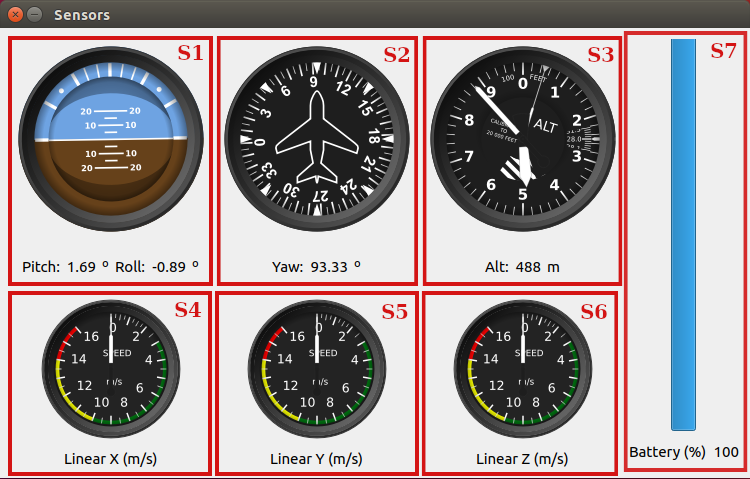
\includegraphics[width=0.8\textwidth]{screenshots/sensors.png}
    \caption{Ventana secundaria de sensores.}
    \label{fig:vent-sens}
\end{figure}

Por último, se presenta un esquema que trata de representar el flujo de información y la secuencia de llamadas del control de vuelo. Este diagrama se muestra en conjunto con el otro control de vuelo y se puede observar en la Figura \ref{fig:control-vuelo}.

\subsection{Control de vuelo: Posicionamiento de aeronave}
El control de vuelo que se encarga del posicionamiento de la aeronave funciona dde forma similar al anterior. El \emph{handler} actualiza la interfaz \emph{Pose3D} con los datos de posicionamiento a través del procedimiento \emph{refreshAPMPose3D()}. Dicho fragmento de código se presenta a continuación (Cód. \ref{listing:refresh-pos}). Los mensajes enviados por cada autopiloto se presentan en la Tabla \ref{table:msg-autopilot}. Los parámetros estos mensajes enviados puede comprobarse en la documentación de MAVLink \cite{mavlink-msg}.

\vspace{2mm}

\begin{longlisting}
\begin{minted} [frame=lines, framesep=2mm, baselinestretch=1.2, bgcolor=LightGray, fontsize=\footnotesize, linenos]{python}

def refreshAPMPose3D(master, pose):
    # get attitude
    if 'ATTITUDE' not in master.messages:
        print("[MAVLink Server] Error: ATTITUDE not received")
    else:
        attitude = master.messages['ATTITUDE']
        yaw = getattr(attitude, "yaw")
        pitch = getattr(attitude, "pitch") * -1
        roll = getattr(attitude, "roll")
        q = quaternion.Quaternion([roll, pitch, yaw])

    # get altitude
    altitude = master.field('VFR_HUD', 'alt', None)
    if altitude is None:
        print("[MAVLink Server] Error: VFR_HUD not received")

    # get GPS position from APM
    latitude = 0
    longitude = 0
    if 'GPS_RAW_INT' not in master.messages:
        gpsStatus = 1
    else:
        gps = master.messages['GPS_RAW_INT']

        latitude = getattr(gps, "lat")/ 10e6
        longitude = getattr(gps, "lon") / 10e6
        GPS_fix_type = getattr(gps, "fix_type")
        sat_visible = getattr(gps, "satellites_visible")

    # refresh the pose3D
    data = Pose3DData()

    data.x = latitude
    data.y = longitude
    data.z = altitude
    data.h = altitude
    data.q0 = q.__getitem__(0)
    data.q1 = q.__getitem__(1)
    data.q2 = q.__getitem__(2)
    data.q3 = q.__getitem__(3)
    pose.setPose3DData(data)

\end{minted}
\caption{Procedimiento \emph{refreshAPMPose3D()}, encargado de leer y actualizar los datos de posición enviados por la aeronave.}
\label{listing:refresh-pos}
\end{longlisting}

\vspace{5mm}

El hilo de posición accede periódicamente a la interfaz y actualiza en la escena la posición de la aeronave. La lectura y escritura sobre la interfaz se protege mediante semáforos para evitar conflictos entre entes. La posición de la aeronave se muestra sobre la escena gracias a la última herramienta de la escena que faltaba por introducir. Esta herramienta aporta un elemento gráfico que puede ser desplegado sobre la escena, y cuya posición se actualiza con la información de la interfaz.

\begin{figure}[h]
    \centering
    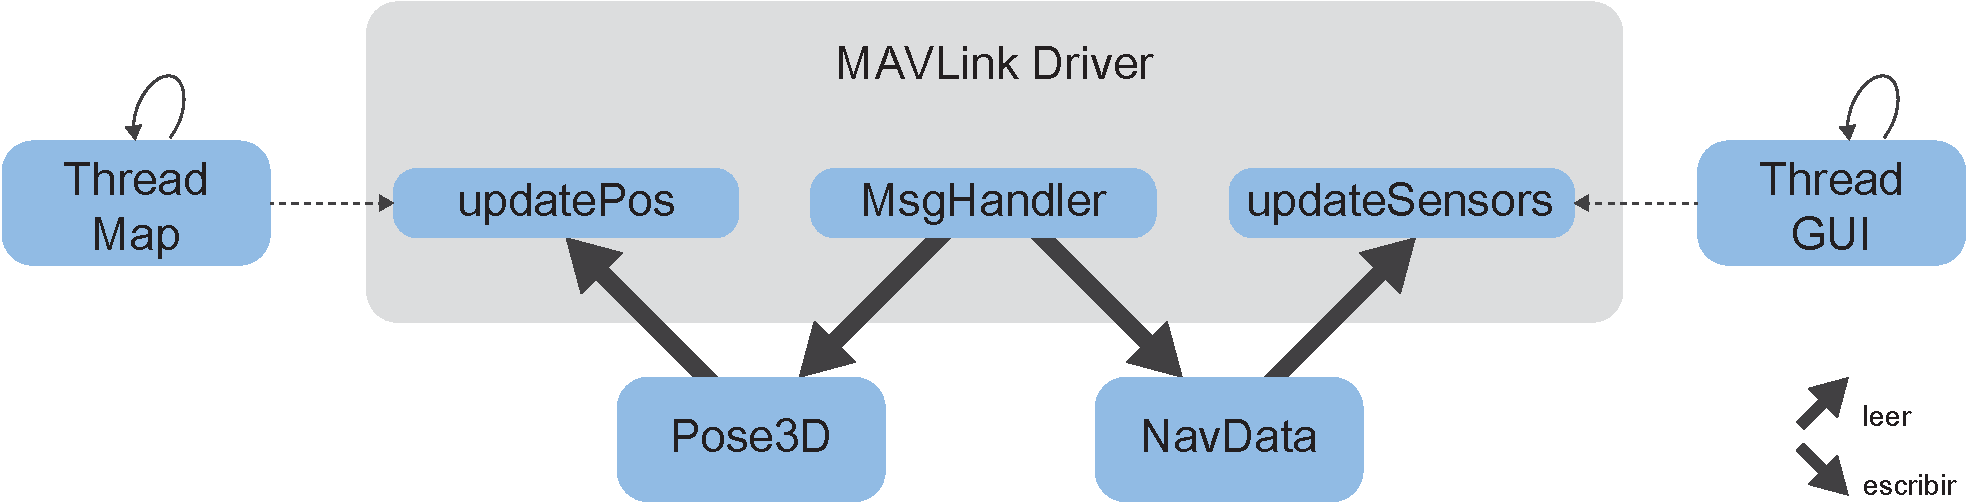
\includegraphics[width=\textwidth]{control-vuelo.pdf}
    \caption{Diagrama del control de vuelo.}
    \label{fig:control-vuelo}
\end{figure}

Finalmente, en la Figura \ref{fig:control-vuelo} se muestra un diagrama con el flujo de información y la secuencia de llamadas de ambas partes del control de vuelo en conjunto.

\subsection{Otros}
Entre otras funciones que incluye el \emph{driver} son el modo de cambio de vuelo, el cambio de velocidad de crucero o el armado y el desarmado. \\
Los modos de vuelo disponibles son:

\begin{itemize}
    \item \textbf{Auto/Mission:} Con el modo automático la aeronave seguirá una misión pre-programada previamente almacenada en el piloto automático.
    \item \textbf{Hold/Loiter:} Este modo ordena mantener la posición, el rumbo y la altitud en el momento de su activación. En el caso de un ala fija, la aeronave realizará círculos alrededor de la posición de activación.
    \item \textbf{Return To Launch:} El modo RTL activa la vuelta de la aeronave al punto de despegue o a un punto fijado como \emph{casa} antes del despegue.
\end{itemize}

El cambio de modo de vuelo se realiza de forma sencilla gracias a la implementación del protocolo MAVLink de pyMavlink. Los procedimientos utilizados por el \emph{driver} se presentan en el Código \ref{listing:modos-vuelo}.

\begin{listing}[h]
\begin{minted} [frame=lines, framesep=2mm, baselinestretch=1.2, bgcolor=LightGray, fontsize=\footnotesize, linenos]{python}

def set_loiter_mode(master):
    master.set_mode("LOITER")
    print('[MAVLink Driver] Flight mode set to LOITER')


def set_rtl_mode(master):
    master.set_mode_rtl()
    print('[MAVLink Driver] Flight mode set to RTL')


def set_auto_mode(master):
    master.set_mode_auto()
    print('[MAVLink Driver] Flight mode set to MISSION')

\end{minted}
\caption{Activación de modos de vuelo.}
\label{listing:modos-vuelo}
\end{listing}

Para el cambio de velocidad de crucero es necesario utilizar otro protocolo de MAVLink. El protocolo de comandos es muy sencillo, pues únicamente es necesario el envío de un mensaje de tipo \emph{COMMAND\_LONG} y esperar su confirmación. La Figura \ref{fig:protocol-cmd} muestra un diagrama del protocolo.

\begin{figure}[h]
    \centering
    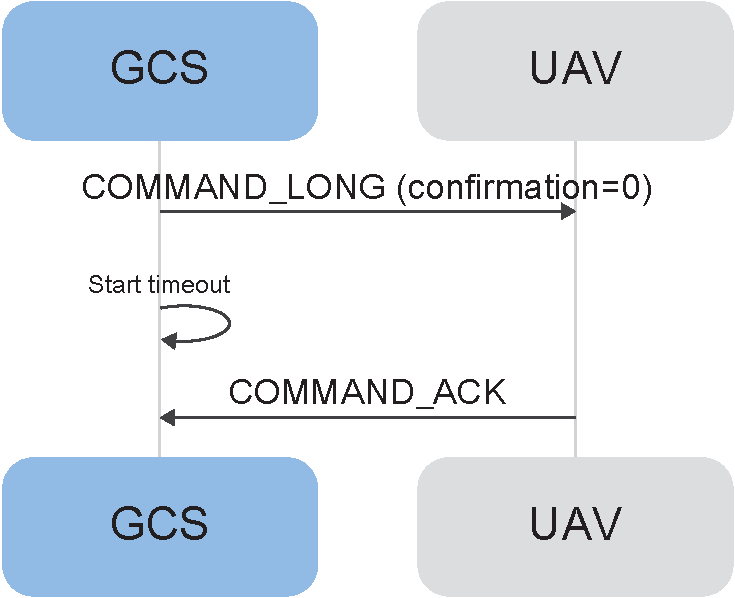
\includegraphics[width=0.5\textwidth]{protoc-cmd.pdf}
    \caption{Diagrama del protocolo de comandos de MAVLink.}
    \label{fig:protocol-cmd}
\end{figure}

La estructura del mensaje \emph{COMMAND\_LONG} se muestra en la Tabla \ref{table:cmd-long}. Para un cambio de velocidad el comando enviado es \emph{MAV\_CMD\_DO\_CHANGE\_SPEED} cuyos parámetros se pueden observar en la Tabla \ref{table:cmd-change-speed}. Para mas detalles acerca de los campos del mensaje se recomienda visitar la documentación de MAVLink \cite{cmd-long}. \\
Por otro lado, la implementación en código del envío del mensaje para el cambio de velocidad se muestra en el Código \ref{listing:cambio-vel}.

\begin{table}[H]
    \centering
    \begin{threeparttable}
        \begin{tabular}{l l l l}
            \toprule
            \thead{Campo} & \thead{Tipo} & \thead{Valores} & \thead{Descripción} \\
            
            \midrule
            target\_system    & uint8\_t  &                    & ID Sistema. \\
            target\_component & uint8\_t  &                    & ID Componente. \\
            command          & uint16\_t & MAV\_CMD           & ID Comando. \\
            confirmation     & uint8\_t  &                    & Nº de transmisión. \\
            param1           & float     &                    & PARAM1. \\
            param2           & float     &                    & PARAM2. \\
            param3           & float     &                    & PARAM3. \\
            param4           & float     &                    & PARAM4. \\
            param5           & float     &                    & PARAM5. \\
            param6           & float     &                    & PARAM6. \\
            param7           & float     &                    & PARAM7. \\
            \bottomrule
            \addlinespace[1ex]
        \end{tabular}
        
    \end{threeparttable}
    
\caption{Mensaje \emph{COMMAND\_LONG} \cite{cmd-long}.}
\label{table:cmd-long}
\end{table}

\begin{listing}[h]
\begin{minted} [frame=lines, framesep=2mm, baselinestretch=1.2, bgcolor=LightGray, fontsize=\footnotesize, linenos]{python}

master.mav.command_long_send(master.target_system,
                                 master.target_component,
                                 mavutil.mavlink.MAV_CMD_DO_CHANGE_SPEED,
                                 0,
                                 0, speed, 0, 0, 0, 0, 0)
                                 
\end{minted}
\caption{Mensaje \emph{COMMAND\_LONG} para el cambio de velocidad de vuelo.}
\label{listing:cambio-vel}
\end{listing}

\begin{table}[H]
    \centering
    \begin{threeparttable}
        \begin{tabular}{l l}
            \toprule
            \thead{Parámetro} & \thead{Descripción} \\
            
            \midrule
            \multirow{2}{*}{Tipo de velocidad} & Airspeed (0), Ground speed (1), \\
             & Velocidad de ascenso (2), Velocidad de descenso (3) \\
            Velocidad          & Velocidad (m/s) \\
            Empuje             & Empuje (\%) \\
            Relativa           & Absoluta (0) o Relativa (1) \\
            param5           & - \\
            param6           & - \\
            param7           & - \\
            \bottomrule
            \addlinespace[1ex]
        \end{tabular}
        
    \end{threeparttable}
    
\caption{Comando \emph{MAV\_CMD\_DO\_CHANGE\_SPEED} \cite{change-speed-cmd}.}
\label{table:cmd-change-speed}
\end{table}

Finalmente, el armado y desarmado de la aeronave también resulta trivial gracias a pyMavlink. El código utilizado por el \emph{driver} se muestra en el siguiente fragmento (Cód. \ref{listing:arm}).

\begin{listing}[h]
\begin{minted} [frame=lines, framesep=2mm, baselinestretch=1.2, bgcolor=LightGray, fontsize=\footnotesize, linenos]{python}

def arm_dissarm(master, arm):
    if arm:
        master.arducopter_arm()
        print('[MAVLinkDriver] Vehicle armed')
    else:
        master.arducopter_disarm()
        print('[MAVLinkDriver] Vehicle disarmed')

\end{minted}
\caption{Armado y desarmado de la aeronave.}
\label{listing:arm}
\end{listing}